%!TEX root = ../template.tex
%%%%%%%%%%%%%%%%%%%%%%%%%%%%%%%%%%%%%%%%%%%%%%%%%%%%%%%%%%%%%%%%%%%%
%% chapter4.tex
%% NOVA thesis document file
%%
%% Chapter with lots of dummy text
%%%%%%%%%%%%%%%%%%%%%%%%%%%%%%%%%%%%%%%%%%%%%%%%%%%%%%%%%%%%%%%%%%%%

\typeout{NT FILE chapter4.tex}%

\chapter{Approach to Elaboration Phase}
\label{cha:elaboration-approach}

% In this chapter, we present our approach to build a scalable and highly modular system with a Hybrid and Flexible Consensus mechanism focused on the permissionless model. We begin by describing a high level system model and architecture and the interactions between the different components of our system. Afterwards, we discuss the design approach focusing on our consensus mechanism and in possible scale-in approaches and open challenges we will address. Then, we present two approaches to the implementation of \mysystem~and discuss how to validate and evaluate our system. Finally, we present the work plan of our solution.

As presented before, \mysystem~is a permissionless solution for scalable ledger using a flexible and hybrid consensus plane, in which different consensus mechanisms will be used alternatively or in combination, by expressing these options with smart contracts. In this chapter we will address the main ideas and initial guidelines for design options, namely system model and architecture \ref{sec:arch}, design approach for system components \ref{sec:approach:design}, prototyping and implementation options \ref{sec:impl_options}, validation and experimental evaluation \ref{sec:experimental-eval} and finally, the work plan \ref{sec:work-plan}.


\section{\mysystem~System Model and Architecture}
\label{sec:arch}

In a high level view, \mysystem~corresponds to a blockchain in which it is composed by different nodes that interact with each other in a \gls{P2P} network. % It is based on the permissionless model with dynamic membership where each node represents a participant of the system and is implemented according to a software architecture with different Service Planes. The objective of \mysystem~is to improve performance on permissionless blockchains by implementing a Self Adaptive consensus mechanism. This mechanism corresponds to an extension of the Consensus Plane which is going to be built on top of already implemented blockchains.
In figure \ref{fig:hyflexchain_architecture}, is presented a high level view of our system model and the different planes that compose it. According to the presented architecture, some components will be leveraged by a base system in which our solution will be implemented, therefore they have a gray background color (the darker color in the Crypto Service Plane means that it is provided by a library). Our focus relies on the following planes: Application Plane, Transaction Management Plane, Hybrid Consensus Plane and Execution Plane. Next, we provide a brief description of their purposes.

\begin{figure}[h]
    \centering
    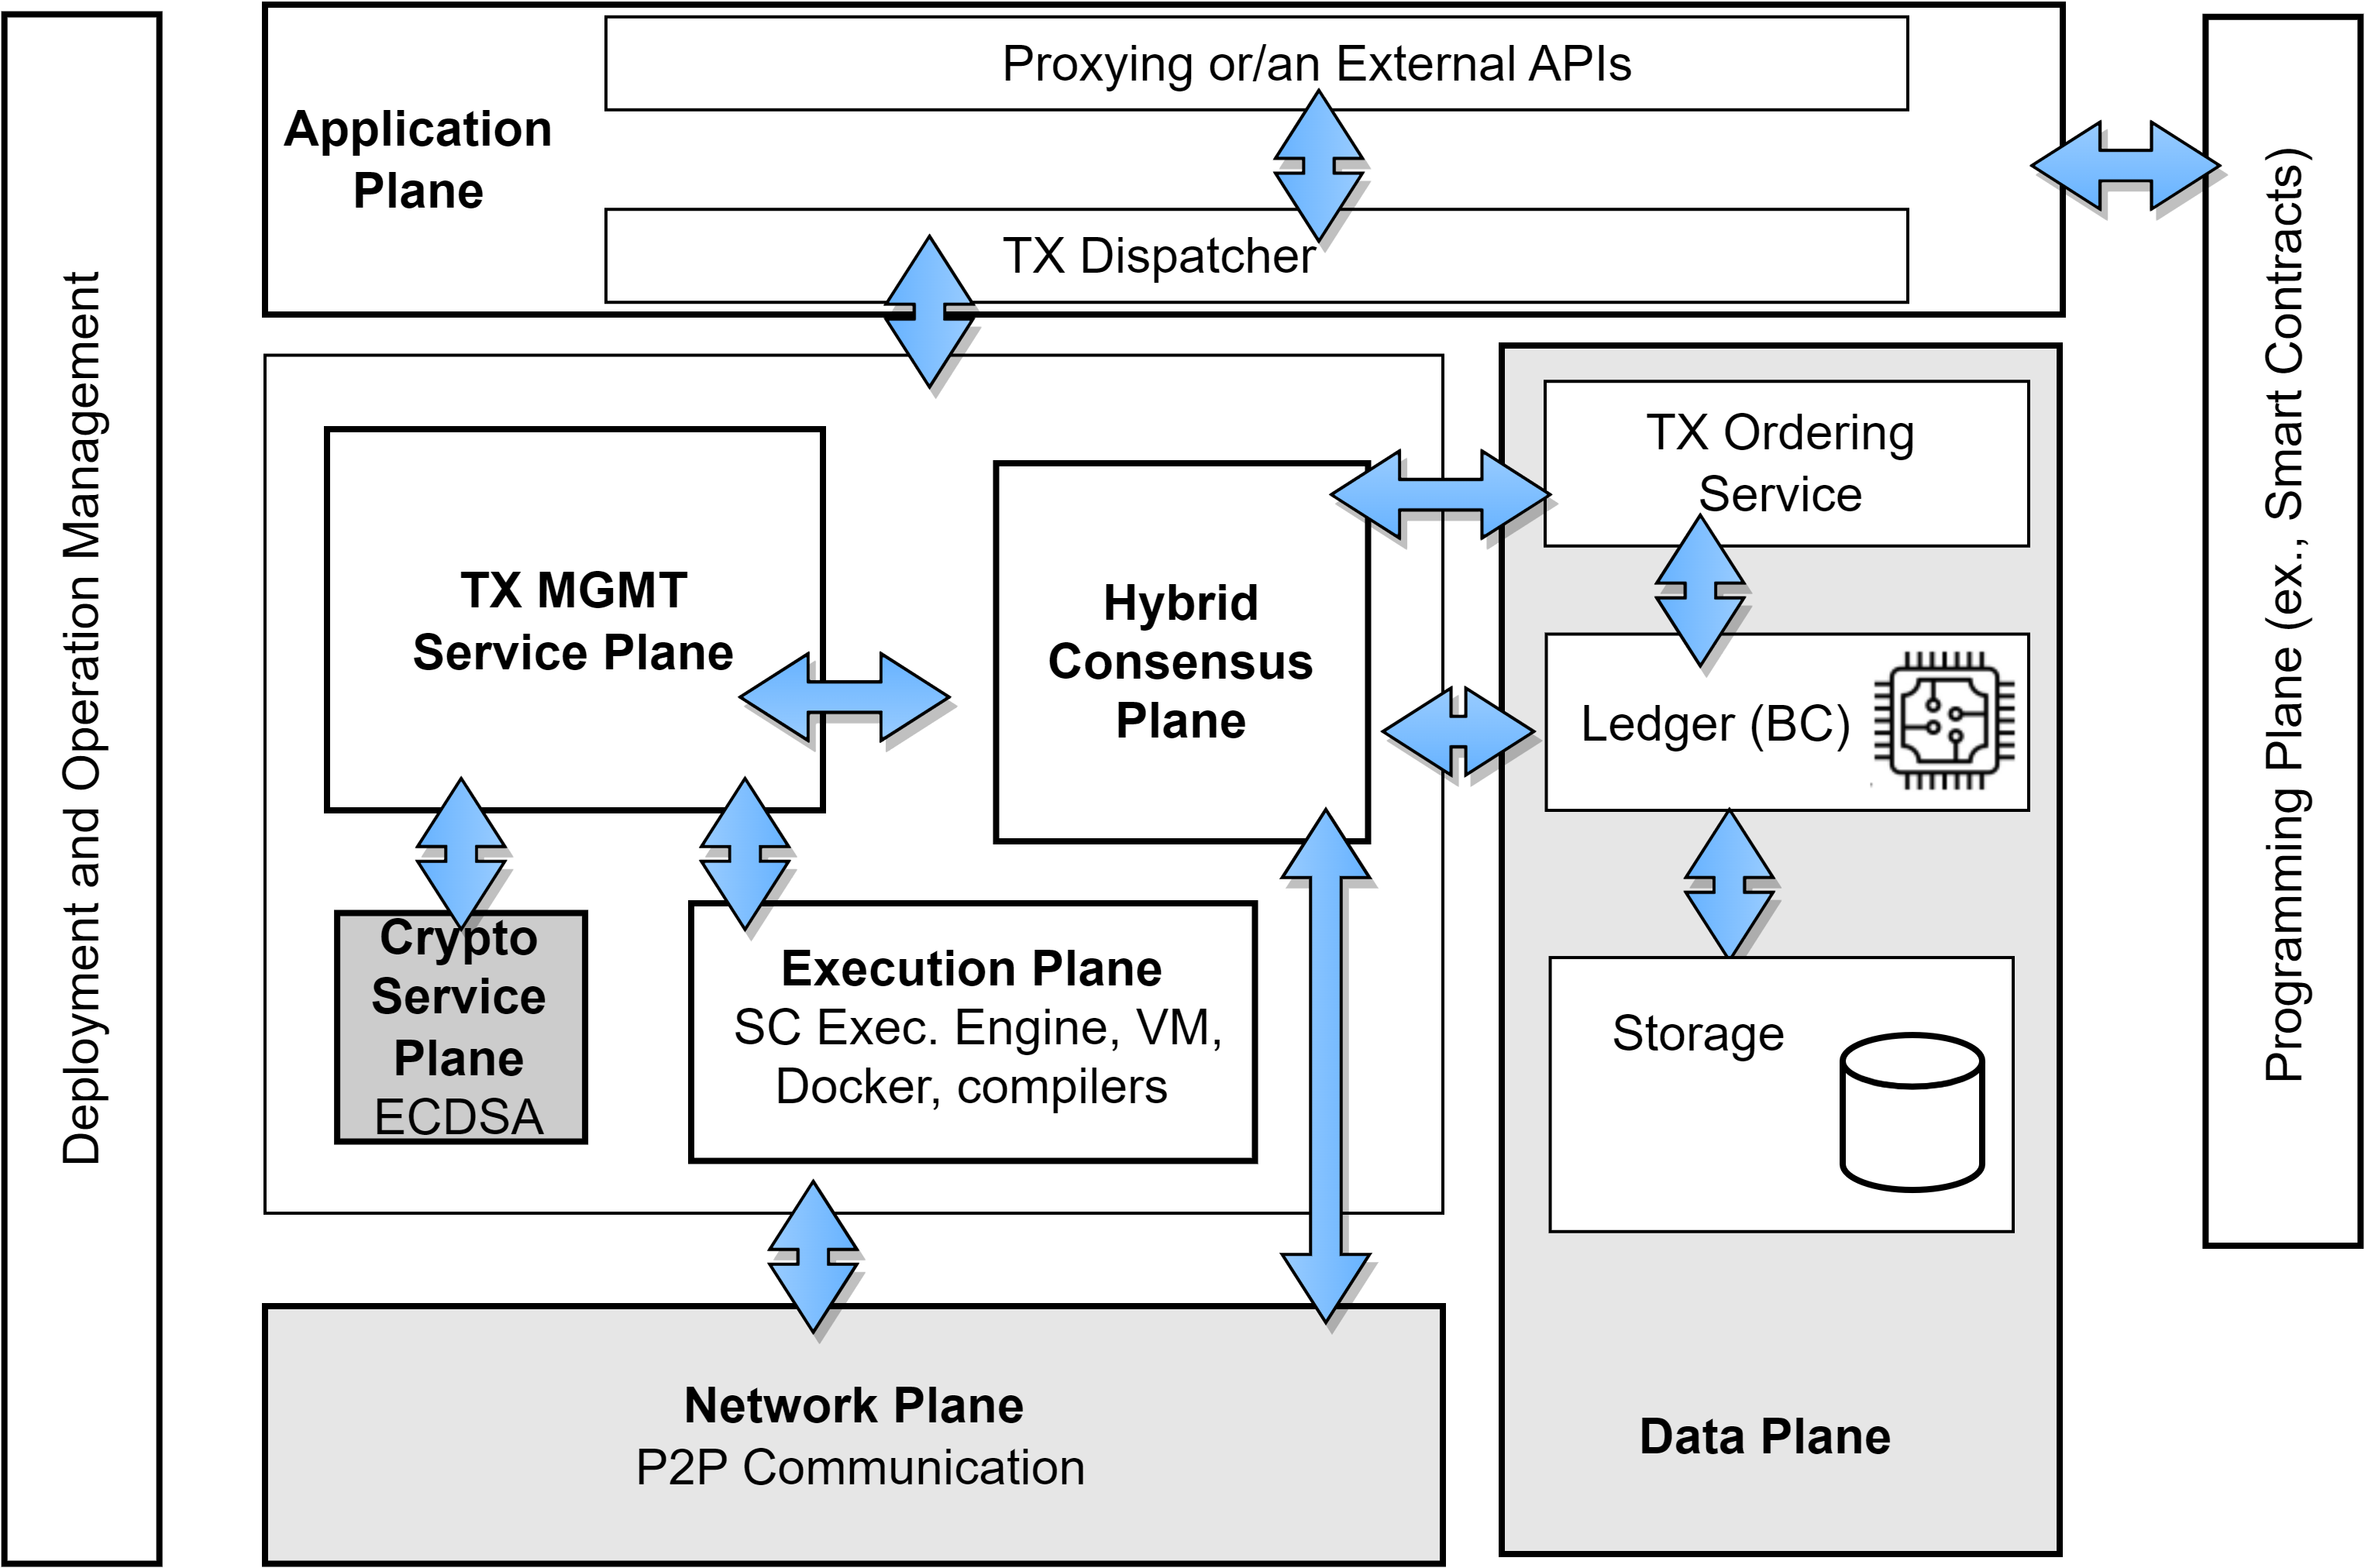
\includegraphics[scale=0.55]{Chapters/Figures/drawio/hyflexchain/hyflexchain_architecture.png}
    \caption{\mysystem~Architecture}
    \label{fig:hyflexchain_architecture}
\end{figure}

\paragraph{Application Plane}
% The Application Plane is responsible for accepting and processing client requests via an external API that is publicly accessed. In this case, a client request corresponds to a transaction that will be submitted to a preliminary validation which will then be dispatched to the Transaction Management Plane in order to be processed. In addition to the transaction's data, this plane is also responsible for accepting embedded smart contracts that will be verified, installed on-chain and executed in the context of a transaction when it is referenced, thus allowing to process Application Specific Validations.

The Application Plane is responsible for accepting and processing client requests via an external API (enabled by REST/HTTPS) endpoint. The provided operations in the API will be organized in three different interfaces: \gls{TI}; \gls{SCMI} and a \gls{LVI}. \gls{TI} corresponds to the client support provided to send transactions that will be submitted to a preliminary validation which will then be dispatched to the Transaction Management Plane. \gls{SCMI} externalized operations to install and revoke smart contracts in a on-chain model. Smart contracts must be validated according to execution constraints and security policies established in the runtime plane and disseminated for the consistent validation of other \mysystem~nodes with special transactions to install and revoke the validated smart contracts in the replicated chain. 

\paragraph{Transaction Management Plane}

This plane is responsible for receiving client transactions via the Application Plane and performing the necessary verifications, such as: transaction verification like ECDSA signatures, smart contract's execution and insertion on blocks which will then be ordered by the Consensus Plane.

\paragraph{Execution Plane}
% The validation, compilation and execution of Smart Contracts is performed by the Execution Plane. It is in this plane that transactions trigger the execution of smart contracts which can imply changes to the system's configuration. In our case, these configurations are boil down to an indication of when a consensus mechanism should be employed, thus having a connection to the Consensus Plane.

This plane is composed by the mechanisms for the validation, compilation and execution of smart contracts. It is in this plane that transactions trigger the execution of smart contracts which can imply changes to the system's runtime settings. These settings affect the consistency model used for blocks that will be ordered under the same consensus verifications which are provided by the different consensus models supported by the Consensus Plane. For the intended purpose, the execution plane contains a virtual execution environment providing testing capabilities for the validation of smart contracts according to security and execution constrained policies (without execution) and execution of validated smart contracts used by transactions. % (when processed in the transaction processing plane).

\paragraph{Consensus Plane}
% This plane deals with the creation of blocks and their ordering in a way that ensures a correct replication of the \gls{DL}. In our solution, we provide a hybrid consensus component in which it is possible to support multiple consensus mechanisms in a flexible way, such as: \gls{PoW}, \gls{PoS}, \gls{PoET} and \gls{PBFT}. The pluggable consensus component \cite{dynamic_reconfiguration_consensus_IoT, research_self_adaptive_consensus} is responsible for providing an interface to access the common primitives of each supported mechanism in a modular and scalable way. Some algorithms (\gls{PoS} and \gls{PBFT}) require a committee in order to be executed, therefore the Sybil Resistant Committee Election procedure is also implemented in this plane.

This plane deals with the creation of blocks and their ordering in a way that ensures a correct replication of the \gls{DL}. In our solution, this plane will be designed to support a hybrid consensus model, using different consensus mechanisms and their protocols. In the consensus plane we support multiple consensus mechanisms, that can be used in a flexible way, targeting on the following models: \gls{PoW}, \gls{PoS}, \gls{PoET} and \gls{PBFT}. By offering a pluggable consensus component \cite{dynamic_reconfiguration_consensus_IoT, research_self_adaptive_consensus}, the consensus plane provides an interface to access the common primitives of each supported mechanism, in a modular way. Some algorithms (\gls{PoS} and \gls{PBFT}) require the existence of formed committees, with anti-sybil resistance capabilities. For the purpose, a core-component in the Consensus Plane will be a Sybil Resistant Committee Election mechanism, with parameterizations to select committees for \gls{PoS} and \gls{PBFT}. Moreover, these committees will be managed in order to achieve fairness conditions with randomized assumptions to rotate or to select committee members with sybil-resistance properties.

\paragraph{Data Plane}
This plane implements the data structures used to record all transaction/blocks in the ledger which then communicates with the storage plane. It is also responsible for saving smart contracts which can then be referenced in future transactions by an identifier in order to be executed. Depending on the type of system we are going to extend, there are different type of structures that we will consider (see \ref{sec:impl_options}).

\paragraph{Network Plane}
The Network Plane is a base plane that provides a way to exchange messages between nodes in a \gls{P2P} network. It is responsible for propagating information (transactions, blocks, consensus messages, etc) to all nodes across the different stages of the system's operation.





% In order to implement \mysystem, we will create a pluggable Consensus Component \cite{dynamic_reconfiguration_consensus_IoT, research_self_adaptive_consensus} that will be able to support different consensus mechanisms in a modular and scalable way. Additionally, we will implement smart contracts with enough expressiveness that provide a flexible way for configuring the consensus mechanism. 




% explorar consenso flexiveis com base em smart-contracts;
% scalable decentralized ledger, utiliza pluggable consenso e permite utilização flexivel de modelos de consenso com base em smart contracts. Poderá melhorar trhougput na utilização simultânea de consensos em várias chains (blockmess).




% \section{System Components}

% In this section, we present the architecture of the system in a more deep level focusing on the interactions between the different Planes presented in the last section. For a better comprehension, we explain the lifetime of a transaction since it is proposed by a client until it is inserted in a block and consequently stored in the ledger.

% Initially, a transaction (possibly including a smart contract) is proposed by a client through an external API which is then dispatched to the Transaction Management Service Plane. In this plane, the transaction's signatures are validated by the Crypto Service Plane using the ECDSA cryptographic scheme. Possibly, smart contracts can be executed in the context of the transaction by the Execution Plane, if it references any. We will implement smart contracts with enough expressiveness in order to reach the objective of allowing a flexible way to apply different consensus mechanisms.

% At this point, the transaction was validated and it is ready to be inserted in a block which is then ordered by the Consensus Plane. In our solution, the Consensus Plane will be a Hybrid component that allows to switch between consensus mechanisms at runtime, meaning that different blocks might be ordered with different consensus mechanisms (see in more detail in section \ref{sec:approach:design}). After reaching consensus, the block is ordered and stored in the Ledger by the Data Plane.



% In this section, we present the architecture of the system in a more deep level focusing on the Consensus Plane and how it relates to the Sybil Resistant Committee Election component in order to perform agreement on the proposed blocks. Also, we discuss how the interaction between those components leads to consensus mechanisms based on elected committees, namely \gls{PoS} and \gls{PBFT}.

% As previously stated, the purpose of \mysystem is to design and implement a Self Adaptive Consensus Plane that integrates multiple consensus algorithms, such as: \gls{PoW}, \gls{PoS}, \gls{PoET} and \gls{PBFT}. In order to support different algorithms in a modular and scalable way, we will adopt a pluggable architecture \cite{dynamic_reconfiguration_consensus_IoT, research_self_adaptive_consensus} in which it will be possible to add more algorithms in the future. This type of architecture will be able to provide a single abstract interface to the consensus Plane in which it will contain all necessary primitives to perform consensus. Then, the interface will call the specific implementation of the current employed consensus algorithm. Additionally, this interface will provide a primitive that allows to switch the current algorithm.

% As discussed in the last chapter in section \ref{sec:rel_work:adversary_model-consensus-consistency}, some consensus algorithms need a committee in order to be executed, which is the case of \gls{PoS} and \gls{PBFT}. In the context of the permissionless model, that committee cannot be statically configured, thus being necessary to perform an election in a secure way. The election procedure must be trustable and fair which means that the elected committee represents all nodes where each node has the same possibility of participating in the committee. In addition, the committee must also be refreshed to avoid collusion and sybil resistant \cite{sybil_attack} so, the election procedure is delegated to a separated component that will take care of the election, namely the Sybil Resistant Committee Election component.

% The Sybil Resistant Committee Election component can support two types of committees based on both \gls{PPoS} and \gls{PBFT} algorithms. In order to support \gls{PPoS}, the election procedure will adopt the solution employed by Algorand \cite{algorand_scaling_bft_cryptocurrencies} in which it is applied a Cryptographic Sortition based on the stake of the participants and takes into account the number of times a node has participated in previous committees. % Also, the use of \gls{VRF} are important for a node to be able to verify if it belongs to the committee without transmitting any message that might compromise it.

% In regard to the implementation and integration of the \gls{PBFT} algorithm, we will adopt a solution that is based on the \gls{CUP} model \cite{cup_model} discussed in section \ref{sec:rel_work:cup}. For generating random committees, we will use the drand API\footnote{Available at: \url{https://drand.love}} which provides a distributed service for generating random numbers in a secure way.



\section{Design Approach for System Components}
\label{sec:approach:design}

In this section we present our design approach specifically focused on the main components we will address, namely: the Application Plane with the $3$ REST APIs, the Hybrid Consensus Plane, smart contract's flexibility and expressiveness and some scale-in approaches and open challenges.

\subsection{Application Plane Components}

% app -> os 3 apis will be implemented as REST API

The \gls{TI} corresponds to an external API that receives transactions proposed by clients. This API will need to verify if the submitted transaction is valid, starting by verifying if the it has the correct syntax and validating the digital signatures. For this, we will use ECDSA signatures which will be provided by an external library. In case of a transaction being considered invalid, it will not be accepted and an error code is returned to the client. 

% is responsible for performing the necessary verifications to all proposed , such as: ECDSA signatures, smart contract's execution and insertion on blocks which will then be ordered by the Consensus Plane.


Regarding the \gls{SCMI}, smart contracts can be submitted through it by any client. Each smart contract (on-chain) will have a unique identifier based on a public-key and digital signature. Only the creator of the smart contract can revoke it on demand, but it will be also considered revoked when the time validity has expired. Only valid smart contracts (consistently stored in finalized blocks) can be used by transactions. Transactions can refer smart contracts to be used in the validation and processing phase. In addition to the transaction's data, this plane is also responsible for accepting embedded smart contracts that will be verified, installed on-chain and executed in the context of a transaction when it is referenced, thus allowing to process Application Specific Validations. 

The operations provided by the \gls{LVI} externalizes the state of the full ledger maintained by the node. The result of operations (that will include ledger searching capabilities) are data view structures derived from the full ledger whose state is obtained by applying all transactions. For performance reasons, pre-computed views may be stored in the storage plane to be accessed in an authenticated fashion. We must notice that permissionless blockchains do not implement this optimization at application level. Miners would need days to reconstruct \gls{UTXO} sets (which can be considered as a “current” view) from the beginning of time. On the other hand, for external wallet-applications the \gls{LVI} provides a necessary support for users to manage their \gls{UTXO}s (representing unspent transactions in the case of cryptocurrency applications) or management of sent or owned digital assets, in the current state of the ledger. In general, a view can be obtained from an arbitrary function of the full ledger (not being necessarily \gls{UTXO} sets). As a piece of data in the storage plane, each view must be determined either implicitly or explicitly by the consensus plane and must allow authentication for the read operation against it. In our design model, views will be supported via replication. For example, Bitcoin \cite{bitcoin}, Ethereum \cite{ethereum} and other popular decentralized cryptocurrencies require all consensus nodes to verify all transactions and so, based on the result of the computation, updating their respective views (\gls{UTXO} sets), locally. In our case, view-states are an implicit output of the Consensus Plane and may be regarded as pre-processed and residing in the storage plane. Assuming it is correctly computed, it represents the computation of an honest set of consensus nodes (each with the same view) providing high availability.


\subsection{Hybrid Consensus Plane}



As previously stated, the purpose of \mysystem~is to design and implement a Hybrid Consensus Plane that integrates multiple consensus algorithms, such as: \gls{PoW}, \gls{PoS}, \gls{PoET} and \gls{PBFT}. In figure \ref{fig:hyflexchain_consensus} we present the architecture of this component.

\begin{figure}[h]
    \centering
    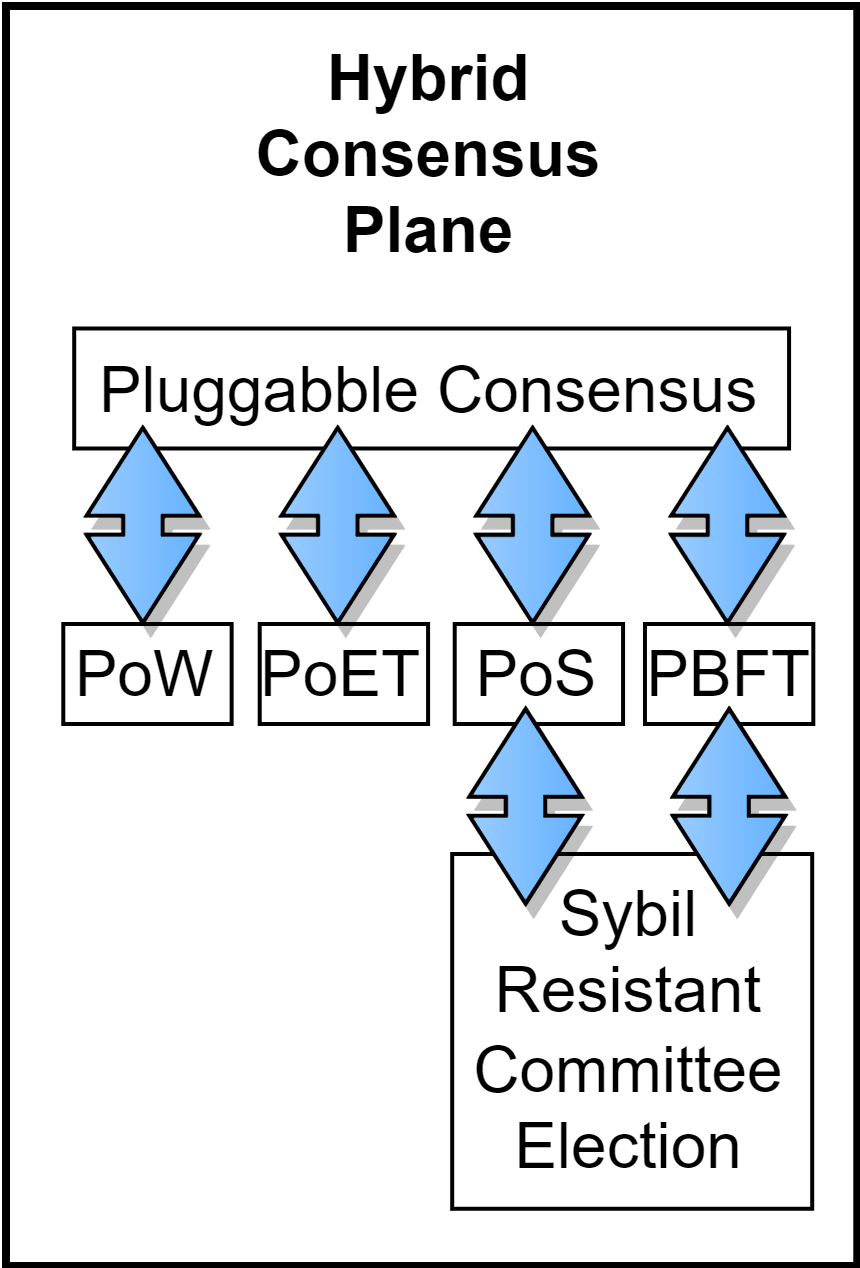
\includegraphics[scale=0.55]{Chapters/Figures/drawio/hyflexchain/hyflexchain_consensus.png}
    \caption{Hybrid Consensus Plane}
    \label{fig:hyflexchain_consensus}
\end{figure}

% In order to support different algorithms in a modular and scalable way, we will adopt a pluggable architecture \cite{dynamic_reconfiguration_consensus_IoT, research_self_adaptive_consensus} in which it will be possible to add more algorithms in the future. This type of architecture will be able to provide a single abstract interface to the consensus plane in the sense that it will contain all necessary primitives to perform consensus. % In this way, when other components interact with this one, they do not need to be aware of which consensus mechanism will be used to order a block, allowing to develop in a modular and scalable way.

% As discussed in the last chapter in section \ref{sec:rel_work:adversary_model-consensus-consistency}, some consensus algorithms need a committee in order to be executed, which is the case of \gls{PoS} and \gls{PBFT}. In the context of the permissionless model, a committee cannot be statically configured, thus being necessary to perform an election in a secure way. The election procedure must be trustable and fair which means that the elected committee represents all nodes where each node has the same possibility of participating in the committee. In addition, the committee must also be refreshed to avoid collusion and to be sybil resistant \cite{sybil_attack}. In this way, the election procedure is delegated to a separated component, the Sybil Resistant Committee Election component, that will take care of the election with the necessary security guarantees.


We will build the consensus plane services on top of underlying blockchain protocols, which we consider as bootstrap slow chains providing a base \gls{PoW} consensus mechanism. Another possibility is to use a base-blockchain already providing a \gls{PoS} model based on fair committees based on the participant's stake but using a randomization scheme to defend from the effect of possible collusions. From the base-slow chain we can form anti-sybil committees for the \mysystem~ which will be used by the consensus plane to support transactions and their aggregations in finalized blocks. For \mysystem~daily operations and supported consensus mechanisms, committees will work with a temporary-validation assumption of two types: elapsed time and a certain number of consecutive participation on block's ordering. To form a new committee from an older one, without leaving gaps of inactivity in between is somewhat tricky. We will tackle this by studying an approach with the following characteristics.

When the new committee is selected, it starts a procedure to be sure that all the elements are committed to start operations in a certain committee-based permissioned consensus model (\gls{PoET} or \gls{PBFT}). A fair sortition of \gls{PoS} committees is already addressed by blockchains we can consider to leverage \mysystem, for example Algorand \cite{algorand}. For \gls{PoW} based committee sortition we will design a mechanism using a cryptographic primitive running a public randomness source (ex. drand \cite{drand}) and a cryptographic sortition protocol based on prior groups and a current list of participants involved in the last $N$ transactions, with $N$ possibly parameterized to correspond to the size of the committees. To enable validators to prove that they belong to the selected subset, they need a public/private key pair to be able to generate a proof using a \gls{VRF}. One open possibility to mitigate the latency in the formation of committees, is to create a set of new committees, to start operations in different future instants of time.

At the same time, a new selected committee is formed and the old committee members previously involved in the type of consensus model initiates a stopping procedure of the existing consensus instance. This would introduce several issues because in transient windows, two (or more) instances of different consensus protocols may be concurrently executing which, in these cases, nodes need to correctly linearize the outputs of the multiple instances. Also, we need to ensure concurrent composition of the multiple instances.

% The Sybil Resistant Committee Election component can support two types of committees based on both \gls{PPoS} and \gls{PBFT} algorithms. In order to support \gls{PPoS}, the election procedure will adopt the solution employed by Algorand \cite{algorand_scaling_bft_cryptocurrencies} in which it is applied a Cryptographic Sortition based on the stake of the participants and takes into account the number of times a node has participated in previous committees. % Also, the use of \gls{VRF} are important for a node to be able to verify if it belongs to the committee without transmitting any message that might compromise it.

% In regard to the implementation and integration of the \gls{PBFT} algorithm, we will adopt a solution that is based on the \gls{CUP} model \cite{cup_model} discussed in section \ref{sec:rel_work:cup}. For generating random committees, we will use the drand API\footnote{Available at: \url{https://drand.love}} which provides a distributed service for generating random numbers in a secure way.



\subsection{Flexible Consensus with Smart Contracts}

% In order to support a flexible consensus mechanism that allows to switch the employed consensus at runtime we will leverage smart contracts. The smart contracts will need enough expressiveness to be able to define rules that indicate when a specific consensus mechanism should be used. For example, one could indicate that a specific transaction must be inserted in a block which must be ordered using the \gls{PBFT} mechanism.

% In fact, this type of approach that uses smart contracts to define the behaviour of the Consensus Plane is extremely powerful in the sense that applications that are built on top of \mysystem~will be able define specific rules that meets their needs. In that case, the responsibility of when each consensus mechanism must be employed is delegated to the application, therefore giving it more control of the underlying system's configurations.

The design of the support for smart contracts will be one of the first tasks in the elaboration phase, together with the design of the APIs at the level of the application plane. Different directions can be explored here.

The first approach will be the use of smart contracts programmed in Java. The bytecodes corresponding to the smart contracts can be executed in a docker component in the execution plane, offering an isolated JVM \cite{jvm} together with pre-established sealed security policy management rules. In this case, we will define smart contracts as implementations of a defined interface model for a Java serializable object (with a $run$ entrypoint function, where the contract will be executed).

Another alternative is to use smart contracts developed using the Solidity programming language \cite{solidity} and using EVM \cite{evm} in a docker component included in the execution plane.


\subsection{Scale-In Criteria and Open Challenges}

% In addition to the above design proposals, we will also try to leverage some scale-in approaches in order to further improve our system performance metrics, namely throughput and latency. For this, depending on the implementation approach (see \ref{sec:impl_options}) we will benefit from parallel chains with the possibility of having different consensus mechanisms in different chains.

% Additionally, \mysystem~will support the \gls{PBFT} consensus mechanism in its Consensus Plane and so, we will adopt a solution that is based on the \gls{CUP} model \cite{cup_model} discussed in section \ref{sec:rel_work:cup}. For generating random committees, we will use the drand API\footnote{Available at: \url{https://drand.love}} which provides a distributed service for generating random numbers in a secure way. In addition to the provided randomness, we will also take into account the nodes that have already succeeded in previous consensus rounds.

Beyond the possibility for applications to use alternatively or in combination, different consensus mechanisms provided by the \mysystem~consensus plane, we will address complementary scale-in conditions, particularly targeting the use of Blockmess \cite{blockmess} as the leveraging solution. Blockmess uses parallel chains to improve the throughput of the system while degrading the finalization time. Then, a possible improvement is the use of the parallel chains to also improve finalization time, as done in Prism \cite{prism}, while the application demands for throughput are low and gradually migrate the use of the parallel chains to increase throughput as the load in the application increases.


While Blockmess estimates the load of the system and creates new parallel chains to adapt application demands, the number of chains the system settles in equilibrium is sub-optimal, as more chains are used than the required. We will study how different parallel chains with different consensus mechanisms can mitigate the problem by complementing the Blockmess solution with a fixed number of parallel chains per consensus-type, effectively creating parallel Blockmess instances usable for different consensus models. If it is known that an application requirements will not drop bellow a certain threshold, we do not need to merge chains bellow a certain number. By not requiring the logic of spawning and merging chains, the fixed parallel chains per consensus types will have a more uniform distribution of load then the original Blockmess. To address this improvement, we must modify the current mechanism used by Blockmess to deterministically allocate transactions to different parallel chains.



\section{Design, Prototyping and Implementation Options}
\label{sec:impl_options}

In this section we explore two alternatives to implement \mysystem. As stated before, \mysystem~will be designed and implemented on top of existing systems as a way to improve their performance by focusing on the consensus plane of those solutions. Then, for each of those approaches we specialize the generic architecture of \mysystem~and discuss the tradeoffs of both solutions, namely through Algorand \cite{algorand_scaling_bft_cryptocurrencies} and Blockmess \cite{blockmess}.

\subsection{Algorand Leveraged Solution}

One of the approaches to develop \mysystem~is through the Algorand blockchain. This blockchain is public and is inserted on the permissionless model that uses \gls{PoS} as the consensus mechanism in order to perform the agreement on the next block to append to the chain. More specifically, this system uses the \gls{PPoS} variant which needs a committee of participants to execute the protocol. % In figure ?? is presented the architecture of \mysystem integrated with Algorand.

Since this system already provides an implementation for the \gls{PoS} consensus mechanism, our objective is to integrate two more mechanisms, such as: \gls{PoW} and \gls{PBFT}. In order to add more consensus mechanisms, we will analyse the code and refactor it to implement a pluggable component which will allow to insert more algorithms and to switch between them at runtime.

Regarding the \gls{PBFT} implementation, it will be necessary to perform a sybil-resistant committee election. In fact, Algorand already does this election procedure, therefore our approach is to try to utilize the elected committee in the \gls{PBFT} mechanism. However, this approach is dependent on the modularity of the election component and how it is integrated with the original consensus algorithm it was developed for. In case of not being possible to reuse that component, we will design an algorithm that randomly chooses a set of nodes based on their correct participation on previous consensus rounds while taking into account a fair election to avoid collusion of nodes.

Note that, the data structures that form the ledger of Algorand are based on a single chain. Based on this, since we are going to develop a component that allows to switch between consensus mechanisms, different blocks will be ordered by different mechanisms. To illustrate this result, we present in figure \ref{fig:hyflexchain_ledger_algorand} an example of the ledger.

\begin{figure}[h]
    \centering
    
\includegraphics[scale=0.5]{Chapters/Figures/drawio/hyflexchain/algorand/hyflexchain_algorand_pluggabble_consensus_chain.png}
    \caption{\mysystem~Algorand Ledger}
    \label{fig:hyflexchain_ledger_algorand}
\end{figure}

Finally, as we already mentioned, our solution will be based on smart contracts with enough expressiveness in order to allow a flexible switch of consensus mechanisms. In this case, Algorand already provides an implementation for smart contracts, therefore our approach corresponds to extend their implementation with the necessary features that we discussed.


\subsection{Blockmess Inspired Solution}

Another approach to implement \mysystem~is inspired by Blockmess, a solution that applies parallel chains in which their number is dynamically adapted to meet application demands, limiting the latency cost and minimizing bandwidth waste in high demand applications. This system works by the assumption that when the rate of proposed transactions is greater than the throughput of the system, it creates more chains and each chain can then spawn even more chains, case it is necessary. This structure forms a tree where each chain represents a path from the \textit{genesis} block and the last block on each chain.

Based on this architecture, our approach will be based on exploring different consensus mechanisms in different chains. In fact, this approach will leverage the algorithm employed by Blockmess to decide in which chain a transaction will be added. Its main idea is for every chain to have a mask and so, the masks decide where transactions can be placed by applying a pattern matching between them and the transaction's identifier.

Our approach consists of using smart contracts to decide which consensus mechanism must be used to order a block in which that transaction is inserted. Since Blockmess does not implement smart contracts and it is a requirement for our solution we will implement that technology which will be focused on providing enough expressiveness in order to define rules for when each consensus mechanism must be used. After deciding the mechanism it is necessary to decide which chain a block with that transaction should be placed. That decision will leverage the algorithm of Blockmess.

\begin{figure}[h]
    \centering
    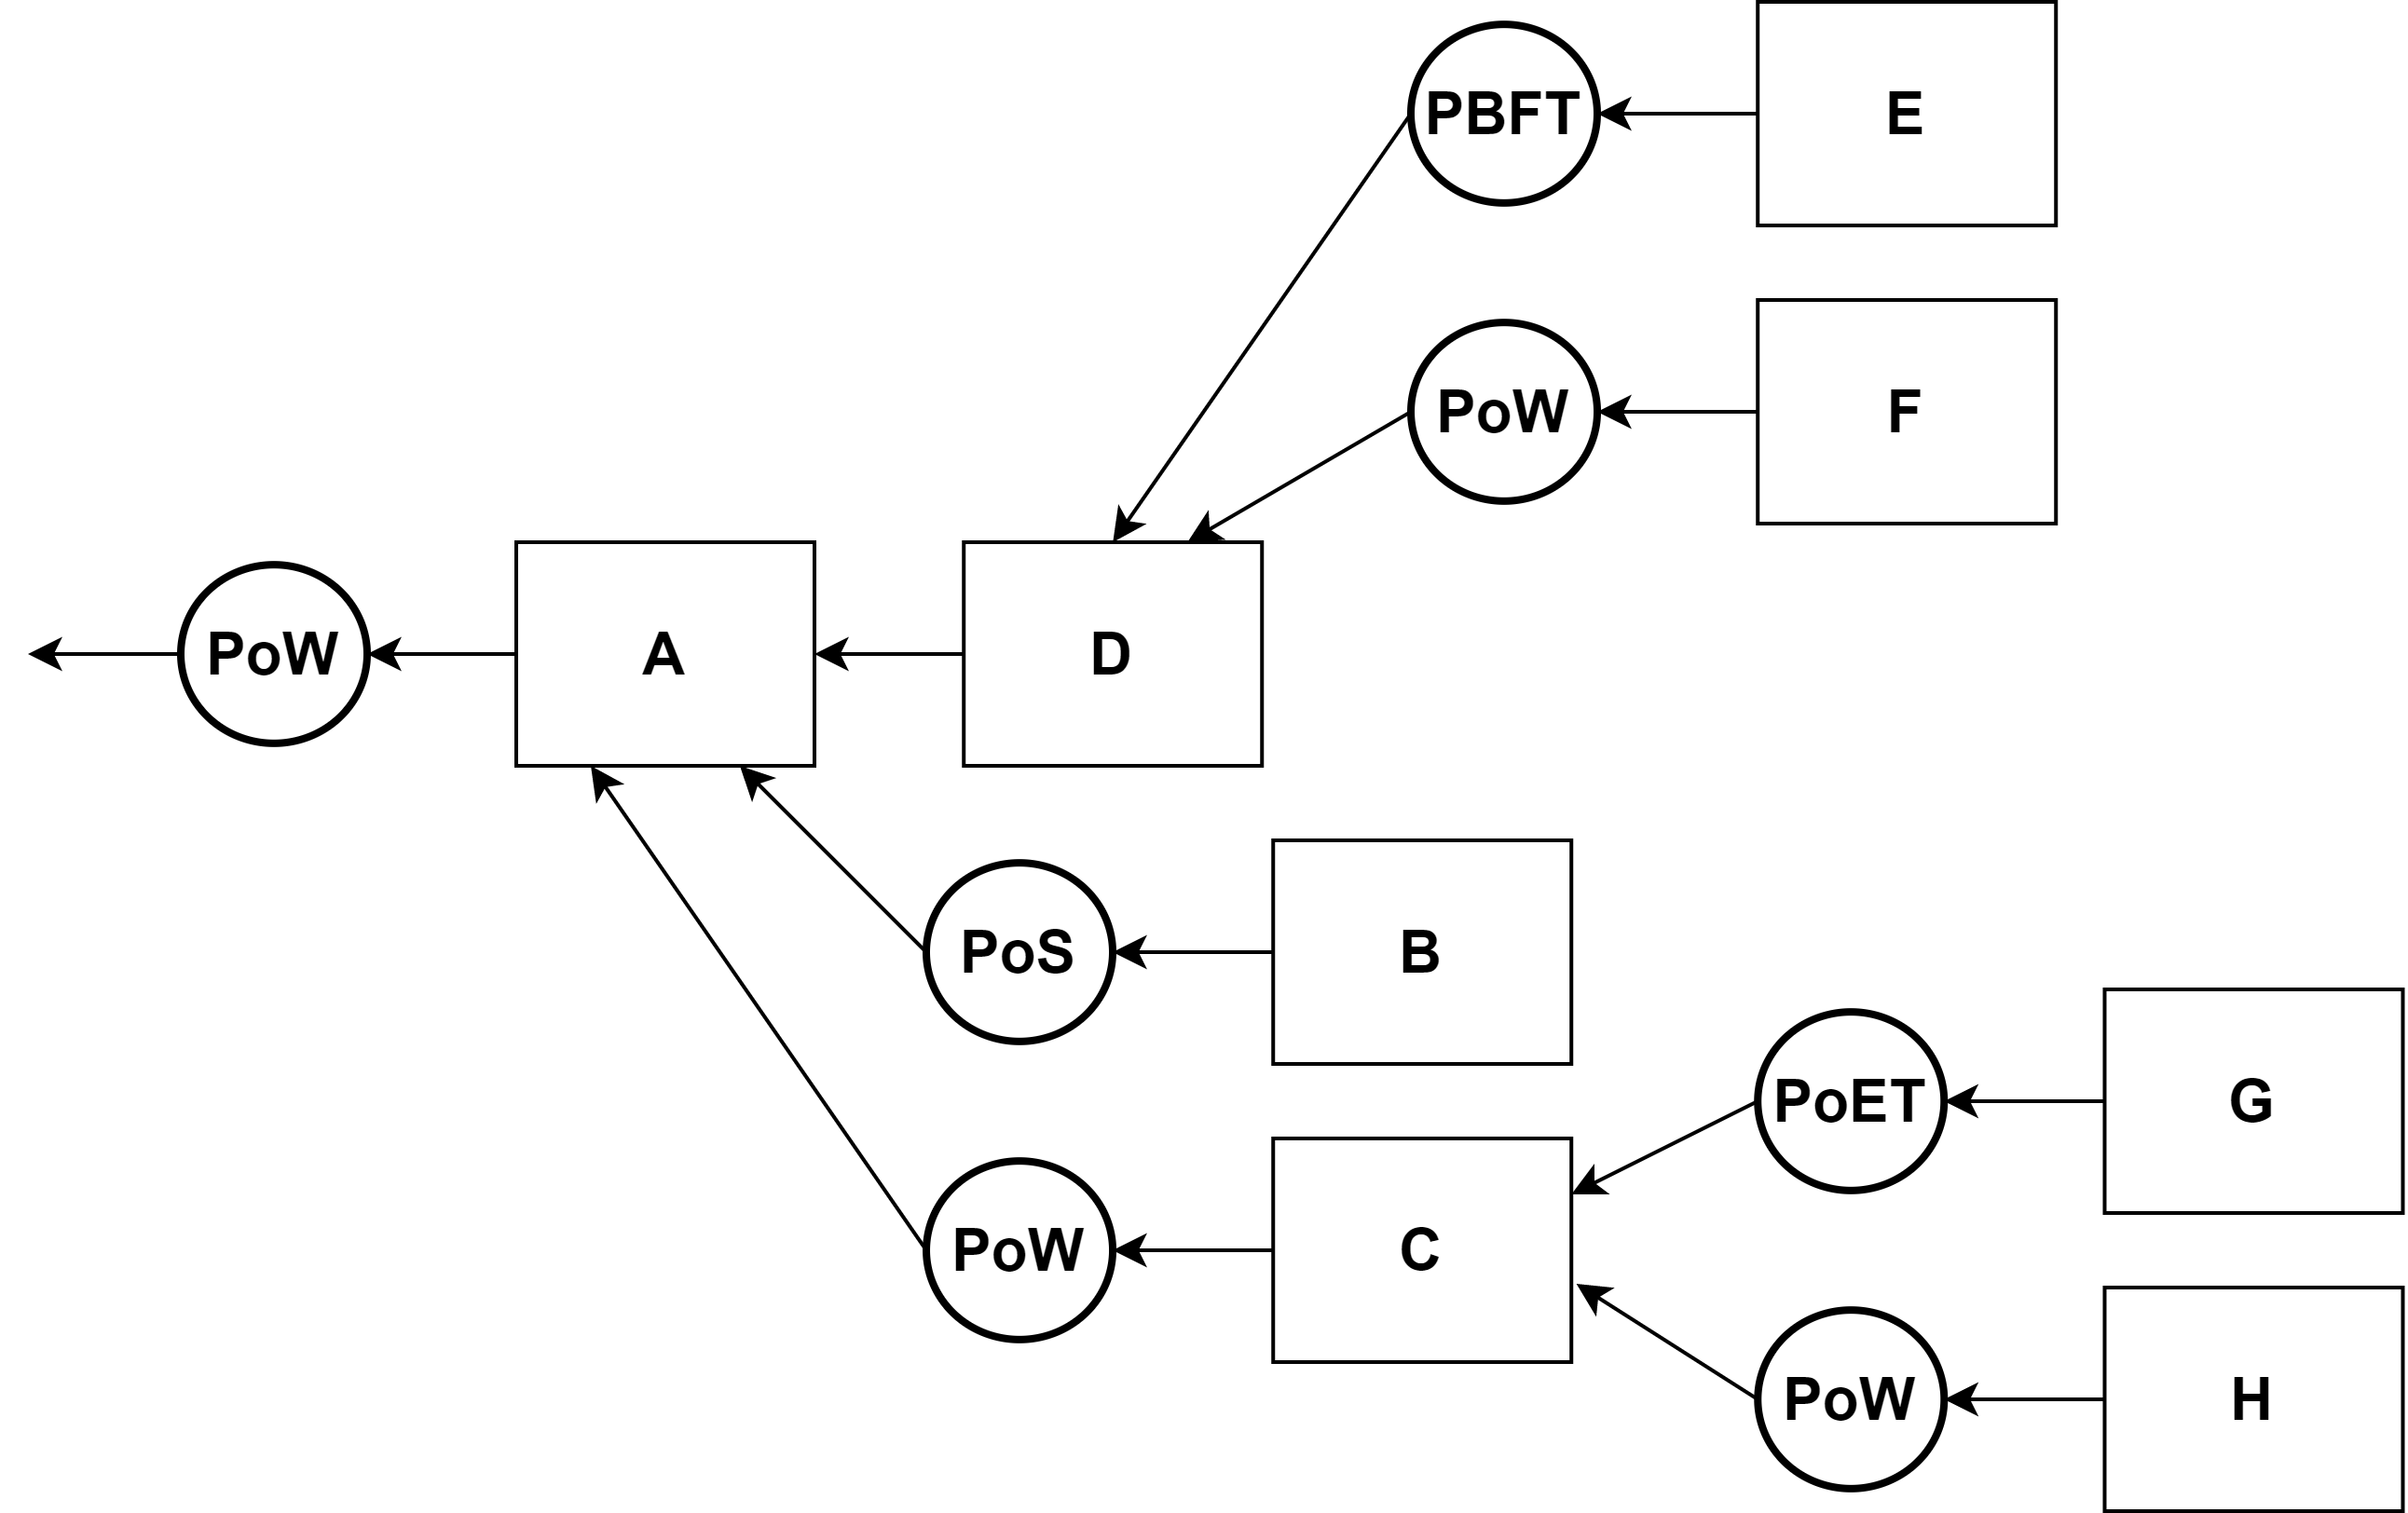
\includegraphics[scale=0.5]{Chapters/Figures/drawio/hyflexchain/blockmess/hyflexchain_blockmess_pluggabble_consensus_chain.png}
    \caption{HyFlexChain Blockmess Ledger}
    \label{fig:hyflexchain_ledger_blockmess}
\end{figure}

In figure \ref{fig:hyflexchain_ledger_blockmess} is presented a possible state of the ledger when applying different consensus mechanisms to different chains. According to the system rules, when the rate of proposed transactions is greater than the throughput of a chain, two more chains are created. Additionally, with our proposed solution we modify that rule to spawn more chains based on the old rule and on different consensus mechanisms. % Therefore, the consensus mechanism of the newly created chains will be same as their parent chain, for example the \gls{PoW} chain was divided into two more chains with the same consensus mechanism.

% Note that, in this type of solution, the state of separate chains is never merged, which can be an issue if transactions reference \gls{\gls{UTXO}} in different chains.

% não há merge de chains, cada node tem todas as chains

% a criaçao de chains é com base no trhourgput ou com base em diferentes consensos.

% problemas: transações que referenciam \gls{UTXO} em diferentes chains

\section{Validation and Experimental Evaluation}
\label{sec:experimental-eval}

The main objective of \mysystem~is to improve performance in permissionless \gls{DL}s and so, we are going to evaluate specific metrics, such as: throughput and blocks' finalization time measurements. These measurements will allow us to attest the benefits of our approach, which in that case can prove that \mysystem~can indeed achieve a higher performance than other permissionless \gls{DL}s. Also, we will analyze possible drawbacks that might appear as a result of our approach.

% Throughput and blocks' finalization time measurements, comparing the benefits of the approach and analyzing possible drawbacks;

Another type of measurements that must be taken into account is the \mysystem~reaction to shifts between consensus models in application demands expressed by the provided smart contracts. In this case, we will test different smart contract's rules and submit a high number of different types of transactions in order to verify if the cost of switching from one type of consensus mechanism with some consistency guarantees to other with different characteristics has an impact on the overall performance of the system. With this, it will be possible to measure the benefits from switching consensus mechanisms at runtime while also taking into account the needed processing to such switches.

%Measurement of HyFlexChain reaction to shifts between consensus models in application demands expressed by te provided smart contracts;

Additionally, we will perform a series of workloads with the purpose of comparing the performance of the system observed by benchmarks at the application level. These workloads will explore the different consensus models that must be employed by the Hybrid Consensus Plane solution. Initially, we will begin with workloads of only one consensus mechanism. Then, execute for $2$, $3$ and $4$ consensus mechanisms. The expectation of the results of those benchmarks is that with the increase of the number of consensus mechanisms on a workload, the higher the overall performance of the system.

% Performance comparison of workloads (observed by benchmarks at application level) using the different consensus models provided by the HyFlexChainHybrid consensus solution.

Initially, we intend to run our experiments on virtual machines provided by the DI-FCT-UNL computation cluster in order to verify and validate our solution with the above test cases. Since we are testing a permissionless \gls{DL}, it will be necessary to conduct tests with a high number of \mysystem~nodes in order to obtain plausible results. Afterwards, we will test our solution in a series of geographically distributed servers based on a global cloud provider infrastructure. With this, we intend to run a total of 200 \mysystem~nodes.


\section{Elaboration Work Plan}
\label{sec:work-plan}

Lastly, we present a schedule for the elaboration plan of the present dissertation during the $2^{sn}$ semester of $2022/2023$. In figure \ref{fig:tasks_calendar} is summarized the elaboration phase work plan. Additionally, in annex \ref{ann:work_plan}, we present a detailed description of planned activities.

\begin{figure}[h]
    \centering
    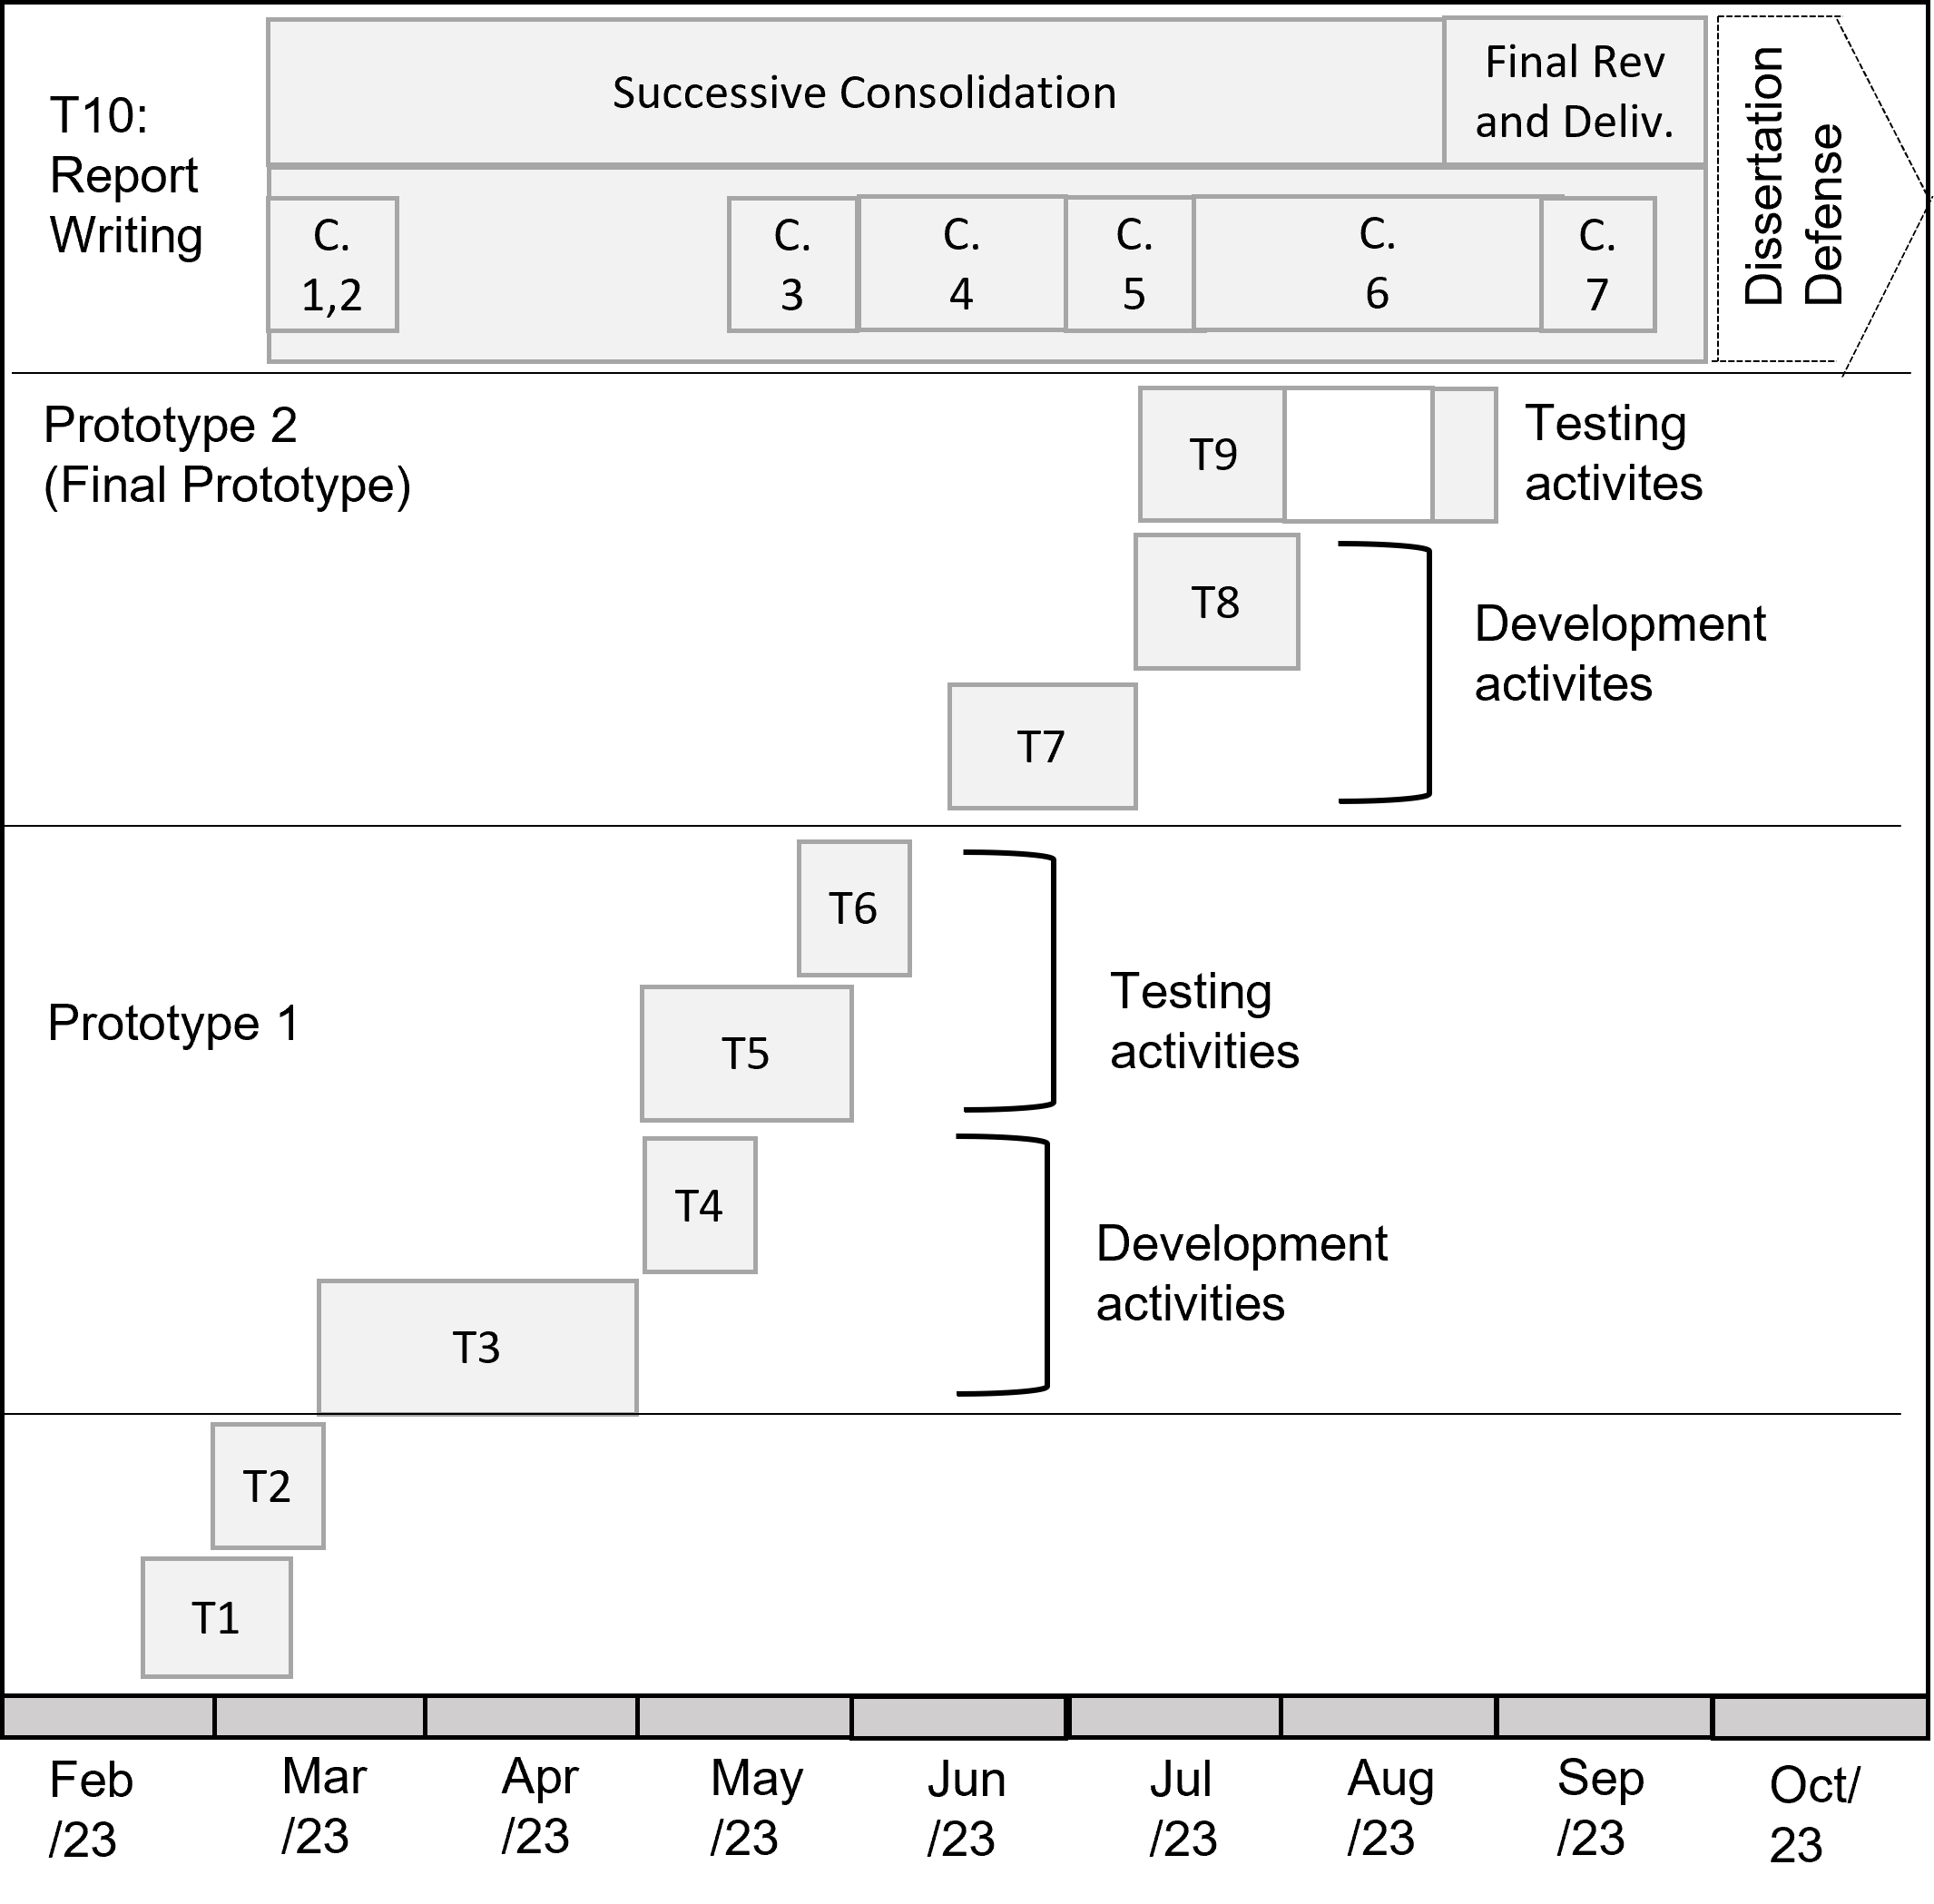
\includegraphics[scale=0.5]{Chapters/Figures/tasks_calendar.png}
    \caption{Planned activities and tasks of the elaboration work plan}
    \label{fig:tasks_calendar}
\end{figure}